%=============================================================================
% Mutual Competition Chapter
% Copyright (c) 2018. Lester James V. Miranda
%
% This file is part of thesis-manuscript.
%
% thesis-manuscript is free software: you can redistribute it and/or modify
% it under the terms of the GNU General Public License as published by
% the Free Software Foundation, either version 3 of the License, or
% (at your option) any later version.
%
% thesis-manuscript is distributed in the hope that it will be useful,
% but WITHOUT ANY WARRANTY; without even the implied warranty of
% MERCHANTABILITY or FITNESS FOR A PARTICULAR PURPOSE.  See the
% GNU General Public License for more details.
%
% You should have received a copy of the GNU General Public License
% along with thesis-manuscript.  If not, see <http://www.gnu.org/licenses/>.
%
% Created by: Lester James V. Miranda <ljvmiranda@gmail.com>
%=============================================================================

\chapter[Selective Feature Extraction via a Mutually-Competitive Autoencoder]{
    \huge Selective Feature Extraction via a Mutually-Competitive Autoencoder
    for Protein Function Prediction
} 
\label{SelectiveChapter}

\par In this chapter, we will introduce the concept of mutual competition,
and demonstrate how it can be used to extract task-relevant features for
protein function prediction. The proposed autoencoder consists of a two-step
operation that ensures retention of neurons best representing the input. This
results to more relevant features, and consequently, better classification.
We begin by describing the autoencoder architecture (Sec.
\ref{MCArchitecture}), then situate it into the prediction pipeline (Sec.
\ref{PFPPipeline}). Then, we outline our experimental set-up (Sec.
\ref{MCExperiments}), and report the results (Sec. \ref{MCResults}). Lastly,
we draw our conclusions and discuss potential avenues for future work (Sec.
\ref{MCConclusions}).


\section{Mutually-Competitive Autoencoder}
\label{MCArchitecture}

Two operations form the core of the mutually-competitive autoencoder as seen in
Figure \ref{schema:mc_autoencoder}: a (1) winner-take-all and (2) sparse
operation. The former constrains the number of active neurons whereas the
latter influences the flow of information throughout the network.

\subsection{Winner-take-all operation}

\par The winner-take-all (WTA) operation retains the top $k$\% neurons in a
given layer based on their activations. Instead of directly proceeding to
reconstruction after the feedforward phase, a percentage of neurons are kept.
This enforces lifetime sparsity\footnote{ Each neuron is activated on a small
subset of examples (\cite{willmore2001characterizing}) } throughout the
extracted features. In this architecture, the value of $k \in
\left[0,1\right]$ serves as a hyperparameter that must be set arbitrarily.

\par The concept of winner-take-all has been studied for the past decade, and
has been applied to numerous fields such as VLSI design and computational
brain models (\cite{maass2000computational}). In artificial neural networks,
WTA can be seen in $k$-sparse architectures (\cite{coates2011sparse,
makhzani2014ksparse, makhzani2015winner}) and sparse coding
(\cite{lee2007efficient, olshausen1996emergence}). In the proposed
autoencoder, WTA is used to focus on neurons with high activations throughout
training. The algorithm for this operation can be seen in Algorithm
\ref{algo:wta}.

\par For each layer, we first perform an affine transformation  (i.e., $h =
\text{ReLU}(\theta^{T}x)$) and take the top-$k\%$ neurons with the highest
activation $h$.  We then store the $k\%$ neurons as winners ($w$), and the
remaining $1-k\%$ as losers ($l$). Keeping a dictionary of winners and losers
is important because the next operation will use this information to adjust the
activations before reconstructing the input data.

\begin{figure}[!t]
  \centering
  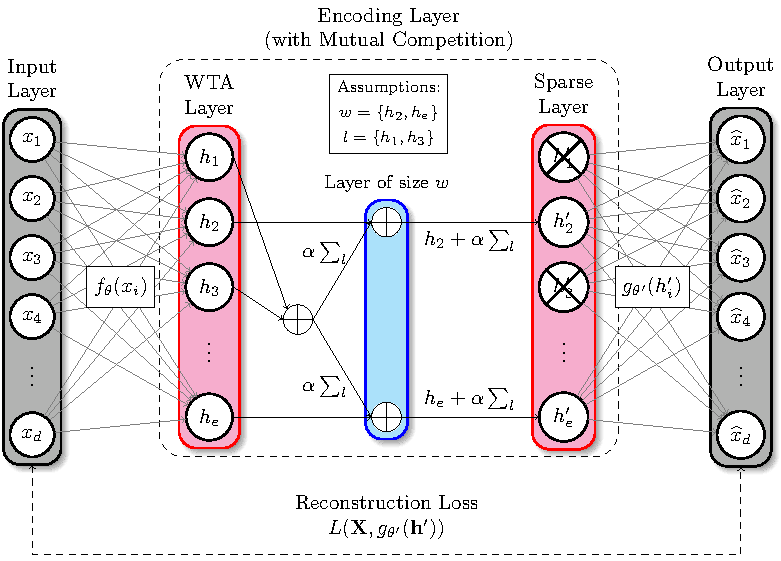
\includegraphics[width=0.65\textwidth]{ch04/mc_autoencoder}
  \caption[Mutually-competitive autoencoder architecture]
  {Mutually-competitive autoencoder}
  \label{schema:mc_autoencoder}
\end{figure}

%=============================================================================
% algo_wta.tex
% Copyright (c) 2018. Lester James V. Miranda
%
% This file is part of thesis-manuscript.
%
% thesis-mansucript is free software: you can redistribute it and/or modify
% it under the terms of the GNU General Public License as published by
% the Free Software Foundation, either version 3 of the License, or
% (at your option) any later version.
%
% thesis-manuscript is distributed in the hope that it will be useful,
% but WITHOUT ANY WARRANTY; without even the implied warranty of
% MERCHANTABILITY or FITNESS FOR A PARTICULAR PURPOSE.  See the
% GNU General Public License for more details.
%
% You should have received a copy of the GNU General Public License
% along with thesis-manuscript.  If not, see <http://www.gnu.org/licenses/>.
%
% Created by: Lester James V. Miranda <ljvmiranda@gmail.com>
%=============================================================================


\begin{algorithm}
    \caption{Winner-Take-All operation}
    \label{algo:wta}
    \begin{algorithmic}[1]
    
    \INPUT Output of last encoding layer $\mathbf{h}$, percent sparsity $k\%$
    \OUTPUT Dictionary of winners and losers, $D = \{\}$

    \item[]
    \State \textit{LayerSize} $\gets$ length($\mathbf{h}$)
    \Comment Get number of units in the layer
    \State \textit{NeuronsToKeep} $\gets k\% * \text{\textit{LayerSize}}$
    \State $D[\text{Winners}] \gets$ first \textit{NeuronsToKeep} in \Call{SortAscendingOrder}{$\mathbf{h}$}
    \State $D[\text{Losers}] \gets$ remaining neurons in \Call{SortAscendingOrder}{$\mathbf{h}$}
    \State \Return $D$
    \end{algorithmic}
\end{algorithm}


\subsection{Sparse operation}

\par The sparse operation allows the winners to ``soak-up'' the activation of
the losers. This is done via an adder controlled by a hyperparameter
$\alpha$. Boosting the energy of the winning neurons affects the
backpropagation path so that weights are optimized in their favor. This
assumes that the winners, due to their high activation, are the relevant
features representing the input data.

\par Selectively manipulating neuron activations encourages competition among
neurons. Throughout training, neurons with consistently high
activations\textemdash i.e. highly-relevant with respect to the output
reconstruction\textemdash are retained. There were some attempts in
maximizing the activation of relevant neurons in the image and text problem
domains: this includes pruning network weights, dropout, and selectively
deleting neurons (\cite{louizos2017learning, chen2017kate, theis2018faster}).
The main difference in this method (in connection with the winner-take-all
operation), is that competition is done via the architecture itself, not as
an objective function or regularizer.

\par Boosting neuron activations is achieved by obtaining the aggregate sum
of the loser activations, and then transferring them to the winner
activations. Meanwhile, the loser activations are set to $0$. Equation
\ref{eqn:sparse_operation} illustrates this process for a layer $\mathbf{h} =
\{h_{w}, h_{l}\}_{i=1}^{d}$ mapped into a ``sparse layer''
$\mathbf{h}^{\prime} = \{h^{\prime}_w, h^{\prime}_l\}_{i=1}^{d}$. In
addition, Algorithm \ref{algo:sparse} describes the whole operation.

\begin{equation}
  \label{eqn:sparse_operation}
  h^{\prime}_{w} = h_{w} + \sum_{i=1}^{e(1-k)}h_{l,i} \quad \text{and} \quad h^{\prime}_l = 0 
\end{equation}

%=============================================================================
% algo_sparse.tex
% Copyright (c) 2018. Lester James V. Miranda
%
% This file is part of thesis-manuscript.
%
% thesis-mansucript is free software: you can redistribute it and/or modify
% it under the terms of the GNU General Public License as published by
% the Free Software Foundation, either version 3 of the License, or
% (at your option) any later version.
%
% thesis-manuscript is distributed in the hope that it will be useful,
% but WITHOUT ANY WARRANTY; without even the implied warranty of
% MERCHANTABILITY or FITNESS FOR A PARTICULAR PURPOSE.  See the
% GNU General Public License for more details.
%
% You should have received a copy of the GNU General Public License
% along with thesis-manuscript.  If not, see <http://www.gnu.org/licenses/>.
%
% Created by: Lester James V. Miranda <ljvmiranda@gmail.com>
%=============================================================================

\begin{algorithm}
    \caption{Sparse operation}
    \label{algo:sparse}
    \begin{algorithmic}[1]
    
    \INPUT Dictionary of winners and losers $D = \{\}$, competition parameter $\alpha$
    \OUTPUT Updated activation of winners and losers $\mathbf{h}'$

    \item[]
    \State \textit{ToAllocate} $\gets$ \Call{Sum}{$D[Losers]$}
    \Comment Sum all activations of loser neurons
    \State $\mathbf{a}_{w} \gets$ $D[Winners]$ + $\alpha$ \textit{ToAllocate}
    \Comment Update activation of winners, $\mathbf{a}_{w}$
    \State $\mathbf{a}_{l} \gets 0$ 
    \Comment Set activation of losers to $0$.
    \State \textbf{return} $\mathbf{h}' = \{\mathbf{a}_{w}$, $\mathbf{a}_{l}\}$
    \end{algorithmic}
\end{algorithm}


\subsection{Hyperparameters and practical considerations}

\par In summary, the combination of the winner-take-all and sparse operations
introduces information bottlenecks when reconstructing the input data. This
should encourage the creation of sparse yet relevant features for
classification. From this design, three hyperparameters can be derived:


\begin{itemize}
  \item \textit{Number of encoding units}, $e$: controls the number of units
  in the hidden layer. If $e > d$, the autoencoder is said to be
  overcomplete, else, undercomplete.
  \item \textit{Number of winners}, $k \in \left[0,1\right]$: controls the
  number of winners retained by the winner-take-all operation.
  \item \textit{Competition parameter}, $\alpha \in \mathbb{R}$: controls the
  intensity to which the loser activations are reallocated to the winners.
  Can range from $10^{1}$ to $10^{2}$.
\end{itemize}

\vspace*{-10pt}
%=============================================================================
% algo-training.tex
% Copyright (c) 2018. Lester James V. Miranda
%
% This file is part of thesis-manuscript.
%
% thesis-mansucript is free software: you can redistribute it and/or modify
% it under the terms of the GNU General Public License as published by
% the Free Software Foundation, either version 3 of the License, or
% (at your option) any later version.
%
% thesis-manuscript is distributed in the hope that it will be useful,
% but WITHOUT ANY WARRANTY; without even the implied warranty of
% MERCHANTABILITY or FITNESS FOR A PARTICULAR PURPOSE.  See the
% GNU General Public License for more details.
%
% You should have received a copy of the GNU General Public License
% along with thesis-manuscript.  If not, see <http://www.gnu.org/licenses/>.
%
% Created by: Lester James V. Miranda <ljvmiranda@gmail.com>
%=============================================================================

\begin{algorithm}[!h]
\caption{Training the mutually-competitive autoencoder network}
\label{algo:mc_training}
\begin{algorithmic}[1]

\INPUT Training examples $\mathbf{X}$, hyperparameters $\langle\alpha, k\%, e\rangle$
\OUTPUT Learned weights, $\theta^{\ast}$

\item[]
\For{\textit{NumEpochs}}
    \State Feedforward propagation: $\mathbf{h} \gets f_{\theta}(\mathbf{X}) =
    \sigma(\theta\mathbf{X}^{T}+\theta_{0})$
    \State $D \gets$ \Call{WinnerTakeAll}{$\mathbf{h}$, $k$}
    \State $\mathbf{h'} \gets$ \Call{Sparse}{$D$, $\alpha$}
    \State Compute output: $\mathbf{\widetilde{X}} \gets 
    g_{\theta'}(\mathbf{h'}) = \sigma(\theta'\mathbf{h'}^{T}+\theta_{0})$
    \State Compute reconstruction error $L$
    \State $\theta^{\ast} \gets$ \Call{Backpropagation}{$L$}
\EndFor
\State \Return $\theta^{\ast}$ 

\end{algorithmic}
\end{algorithm}



\section{Protein Function Prediction Pipeline}
\label{PFPPipeline}

\par The entire protein function prediction model consists of two stages: (1)
a \textit{feature extraction} stage that contains the mutually-competitive
autoencoder, and a (2) \textit{multi-label classification} stage that assigns
each protein sample to its respective set of functions.\footnote{This
pipeline is similar to the one we implemented using the stacked denoising
autoencoder in Chapter \ref{SDAEChapter}} During training, the model learns
the parameters $\theta$ and $W$ for the two stages separately. At inference,
matrix operations are applied to transform the input data and predict protein
functions. Figure \ref{schema:traintest_mc} shows the training and test
phases.

%\newpage
\begin{itemize}
  \item \textit{Training phase:} our goal during training is to learn the
  parameters $\theta$ for the feature extractor, and $W$ for the classifier.
  We simply implement the traditional training scheme for autoencoders (Alg.
  \ref{algo:autoenc}), and minimize the mean-square error, $L$ (Eq.
  \ref{eqn:loss_fe}). Then, we minimize the L2-SVM loss (Eq.
  \ref{eqn:loss_clf}) for our classifier:
  \begin{align}
    % Feature Extractor Loss
    \label{eqn:loss_fe}
    L(\mathbf{X},g_{\theta^{\prime}}(\mathbf{h}^{\prime})) &=
      \dfrac{1}{2}(\mathbf{X} - g_{\theta^{\prime}}(\mathbf{h}^{\prime}))^{2}\\
    % Multilabel classifier loss
    \label{eqn:loss_clf}
    J(\mathbf{X}^{\prime}, \widehat{\mathbf{Y}}, \mathbf{Y}) &= \sum_{\widehat{\mathbf{y}}_i \neq \mathbf{y}_{i}} \text{max}(0, W^{T}_{\widehat{\mathbf{y}}_{i}} \mathbf{x}_{i}^{\prime} - W^{T}_{\mathbf{y}_i}\mathbf{x}^{\prime}_i + \Delta)^2
  \end{align}
  \item \textit{Test phase:} upon learning the parameters $\theta^{\ast}$ and
  $W^{\ast}$, we pass our test data into the feature extractor
  $f_{\theta^{\ast}}$ (Eq. \ref{eqn:encoder_mc})\textemdash turning-off the WTA and sparse
  operations\textemdash and classify the resulting features using
  $\mathcal{H}$.
  \begin{align}
    % Encoder equation
    \label{eqn:encoder_mc}
    f_{\theta^{\ast}}(\mathbf{X}_{ts}) = \theta^{\ast T} \mathbf{X}_{ts} + \theta_{0}^{\ast}
  \end{align}
\end{itemize}

\begin{figure}[!h]
  \centering
  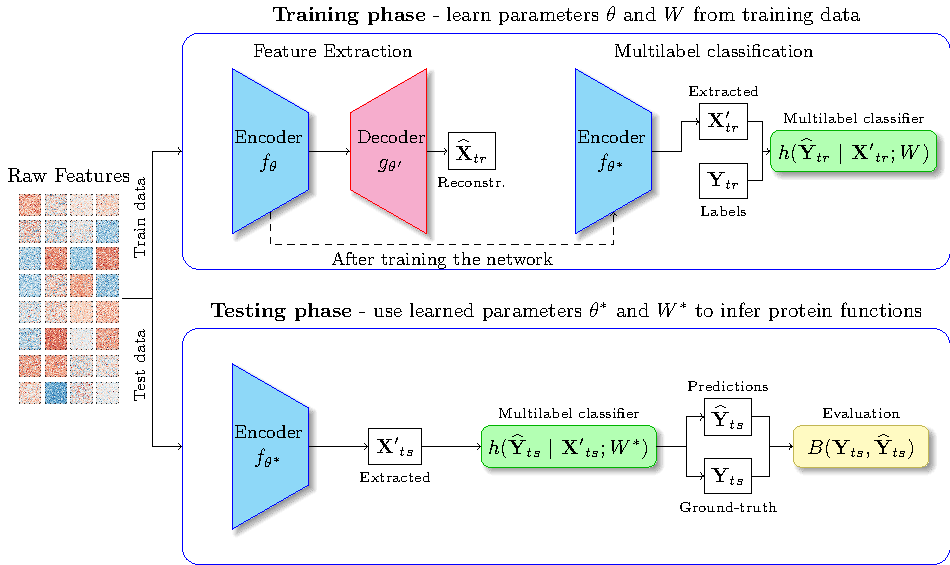
\includegraphics[width=0.90\textwidth]{ch04/schema_traintest}
  \caption[Protein function prediction pipeline]{Protein function prediction
  pipeline for the mutually-competitive autoencoder}
  \label{schema:traintest_mc}
\end{figure}

\newpage
\subsection{Evaluation metrics}

After testing, we now have a set of predictions $\mathbf{\widehat{Y}}_{ts}$
to compare against a held-out ground-truth labels $\mathbf{Y}_{ts}$. To
evaluate the performance of the prediction model, we will use the following
metrics\footnote[2]{\textit{tp}: true positive, \textit{fp}: false positive,
\textit{tn}: true negative, \textit{fn}: false negative}:

\begin{align}
    \text{Hamming Loss (H)} &= \dfrac{1}{N \cdot L} \sum_{i=1}^{N} \sum_{j=1}^{L}
    \text{XOR}(y_{ij}, \widehat{y}_{ij}) \\
    \text{Precision (P)} &=
    \dfrac{1}{N}\sum_{i=1}^{N}\dfrac{|\mathbf{\widehat{y}}_{i} \cap
    \mathbf{y}_{i}|}{|\mathbf{\widehat{y}_{i}}|} = \dfrac{tp}{tp + fp} \\
    \text{Recall (R)} &=
    \dfrac{1}{N}\sum_{i=1}^{N}\dfrac{|\mathbf{\widehat{y}}_{i} \cup
    \mathbf{y}_{i}|}{|\mathbf{\widehat{y}_{i}}|} = \dfrac{tp}{tp + fn} \\
    \text{F-score (F)} &=
    \dfrac{1}{N}\sum_{i=1}^{N} \dfrac{2 | \mathbf{\widehat{y}}_{i} \cup
        \mathbf{y}_{i}|}{|\mathbf{\widehat{y}}_{i} | + |\mathbf{y}_{i}|} =
        \dfrac{2 (\text{P} \cdot \text{R})}{\text{P} +
        \text{R}}
\end{align}

\par We will also compute for a fifth metric, the Area Under the ROC Curve
(AUROC), to serve as proxy for accuracy. Together with the Hamming loss and
F-score, the model will be evaluated and compared to other works. Lastly, the
Precision-Recall score will determine the quality of our model in terms of
sensitivity and specificity. This time, we will obtain the micro, macro, and
samples average for the AUROC and F-score, enabling us to further gauge model
performance.

\section{Experimental Set-up}
\label{MCExperiments}

There are two experimental themes in this work. First, we characterized the
proposed autoencoder by examining how each hyperparameter, $\langle e, k\%,
\alpha \rangle$, affects the classifier's ability to discriminate samples.
Then, we conducted experiments to test our hypotheses on feature relevance and
prediction performance. A summary of all experiments can be seen in Tables
\ref{exp:hyperparameter} and \ref{exp:key_results}.

\begin{table}[h]
  \centering
  \caption{Summary of experiments for autoencoder characterization}
  \label{exp:hyperparameter}
      \begin{tabular}{@{}rp{0.65\textwidth}@{}}
          \toprule
          Hyperparameter                      & Description \\ \midrule
          Nb. of encoding units, $e$    & Test overcomplete and undercomplete configurations.\\
          Nb. of winners, $k\%$     & Sweep $k$-values in the range $\left[ 0,1\right]$\\
          Competition parameter, $\alpha$ & Rough search from $\num{1e-3}$ to $\num{1e3}$\\ \bottomrule
      \end{tabular}
\end{table}

\begin{table}[t]
  \centering
  \caption{Summary of experiments for analysis and benchmarking}
  \label{exp:key_results}
  \begin{threeparttable}
      \begin{tabular}{@{}rp{0.65\textwidth}@{}}
          \toprule
          Experiment                      & Description \\ \midrule
          Estimating feature relevance    & Obtained a distribution of feature scores by growing a decision tree on the features\tnote{1} \\
          Model quality         & Plotted ROC and PR curves for both
          datasets\tnote{2}\\
          Benchmark analysis     & Compared proposed model against other
          techniques in literature\tnote{3}\\
          Ablation test                   & Investigated the necessity of adding
          mutual competition in the traditional autoencoder\\\bottomrule
      \end{tabular}
  \begin{tablenotes}
      \footnotesize
      \item[1] Score distribution is normalized and averaged across all labels.
      \item[2] ROC - Receiver Operating Characteristic, PR - Precision--Recall
      \item[3] Friedman's test \parencite{friedman1937use} and post-hoc Bonferroni-Holm test \parencite{holm1979simple}
      were employed to measure statistical significance as recommended by \cite{demsar2006statistical}.
  \end{tablenotes}
  \end{threeparttable}
\end{table}

\par Lastly, Table \ref{exp:implementation} describes the implementation
environment for running the tests. The neural network was trained on an
NVIDIA Titan X (Pascal) GPU while the classifier was fitted using an Intel
Xeon 2.2GHz CPU. The majority of the code was written in Python 3.6.X using
the \href{https://www.tensorflow.org/}{Tensorflow} and
\href{https://keras.io/}{Keras} package\footnote{For more information on how
the classifier was trained and how the software package was used, please see
the Appendix}.

\begin{table}[!h]
  \centering
  \caption{Experimental environment}
  \label{exp:implementation}
  \begin{threeparttable}
  \begin{tabular}{@{}rp{0.70\textwidth}@{}}
      \toprule
      Environment                    & Value                                             \\ \midrule
      \textit{Validation and testing}                                                    \\
      Number of trials               & 10: mean and std. dev. reported                   \\
      Train--validation--test split  & 50--30--20                                        \\ \cmidrule{1-2}
      \textit{Hardware dependencies}                                                     \\
      Number of cores\tnote{1}       & 10 in use (40 maximum)                            \\
      CPU                            & Intel Xeon 2.2GHz: Classifier training            \\
      GPU                            & NVIDIA Titan X (PASCAL): Neural network training  \\ \cmidrule{1-2} 
      \textit{Software dependencies}                                                     \\
      Package Name                   & PFPredict\tnote{2}                                \\
      Language                & Python 2.7, 3.6 (compatible to both versions)            \\
      Libraries               & Tensorflow 1.2.1, Keras 2.1.2, Numpy 1.14.2              \\ \bottomrule
  \end{tabular}
  \begin{tablenotes}
    \footnotesize
    \item[1] We implemented a distributed scheme for training the classifier.
    Please see Appendix \ref{AppendixDistributed}.
    \item[2] PFPredict is a small package we developed for the mutually-competitive autoencoder.
    Please see Appendix \ref{AppendixPFPredict}.
  \end{tablenotes}
  \end{threeparttable}
\end{table}

\section{Results and Discussion}
\label{MCResults}

\par This section presents the experimental results listed in Tables
\ref{exp:hyperparameter} and \ref{exp:key_results}. Again, we'll first
investigate how different hyperparameter settings, namely, $e$, $k\%$, and
$\alpha$, affect the model's predictive performance for the two protein
benchmarks. Then, we'll test our claims using various experiments listed in
Table \ref{exp:key_results}. Remember that our main hypothesis states that the
features extracted by the mutually-competitive autoencoder are
\textit{relevant}, and should result to better predictions for the multilabel
classifier.

\newpage
\subsection{Characterizing the autoencoder model}

In this experiment, we tested how different hyperparmeter settings affect the
model as a whole. We'll be using the Area under the ROC curve as our main
metric. The procedure is simple: change a specific hyperparameter
$\mathcal{P}$ and measure the resulting AUROC while keeping other variables
constant. We redo this process for different values of $\mathcal{P}$. 

\par Note that these experiments were performed to find a pattern on model
behavior given a dataset. Once these patterns are determined, a fine-search
(\cite{bergstra2012random}) is conducted to get the actual values. The
implementation details can be seen in Appendix \ref{AppendixImplementation}.

\subsubsection{Experiments on the Yeast Dataset}

Figure \ref{results:mc_benchmark_yeast} shows the results for Yeast. Recall
that validation set performance should always be lower than training set
performance, as the former simulates unseen samples. Here we can observe the
following:

\begin{itemize}
  \item An overcomplete autoencoder ($e=500$) gives the optimal validation
  set performance. However, adding more hidden units tends to overfit the
  model.
  \item The amount of winners to keep should not be too high ($k=1.00$) nor
  too low ($k=0.00$). Here, we see an optimal value in the middle range
  ($k\in\left[0.33, 0.67\right]$).
  \item The value of $\alpha$ should not be excessively high nor excessively
  low. A value between \num{1e0} to \num{100} should suffice.
\end{itemize}

\begin{figure}[!h]
  \centering
  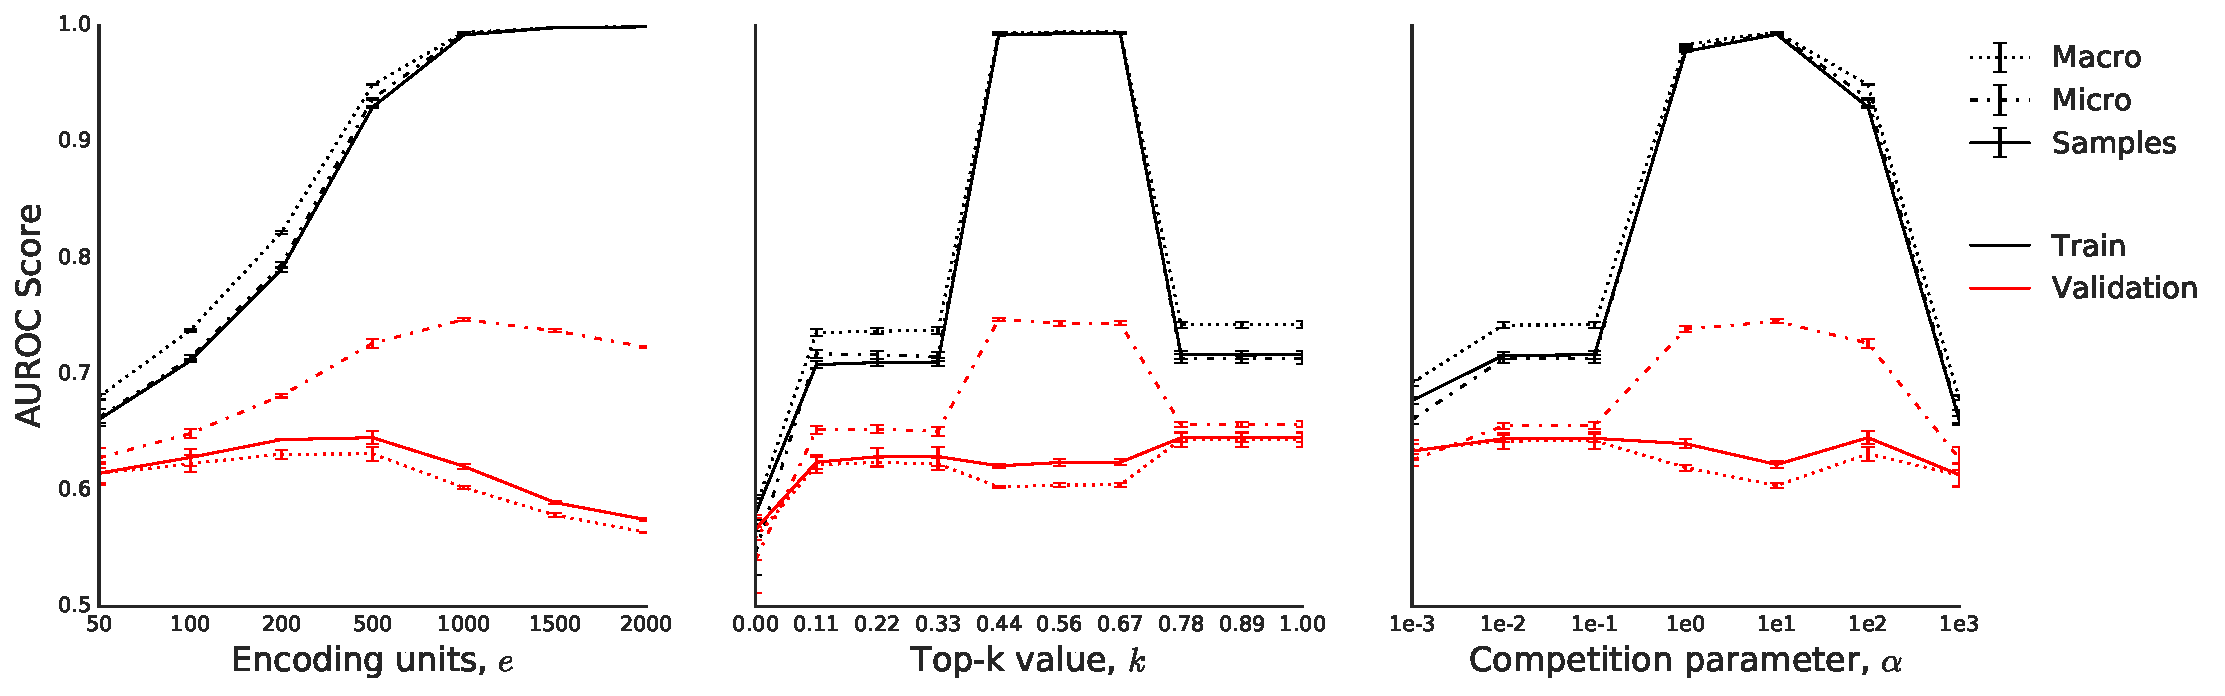
\includegraphics[width=0.95\textwidth]{ch04/hyperparams_yeast}
  \caption{Model behavior on the Yeast Dataset}
  \label{results:mc_char_yeast}
\end{figure}

\subsubsection{Experiments on the Genbase Dataset}

Figure \ref{results:mc_char_genbase} shows the results for Genbase. A similar
procedure was performed for both training and validation data. We can infer
the following from the plots:

\begin{itemize}
  \item An undercomplete autoencoder ($e\in\left[50,100\right]$) gives the
  optimal validation set performance. A large value can damage the model (e.g.,
  $e=2000$).
  \item Similar to the Yeast dataset, the amount of winners should be
  moderated. Although lower values are preferred, setting them too low can
  potentially damage the model.
  \item The competition parameter $\alpha$ can be set at a lower value (around
  $\alpha \in \left[1,10\right]$). Increasing this value further only gives
  marginal benefits.
\end{itemize}

\begin{figure}[!h]
  \centering
  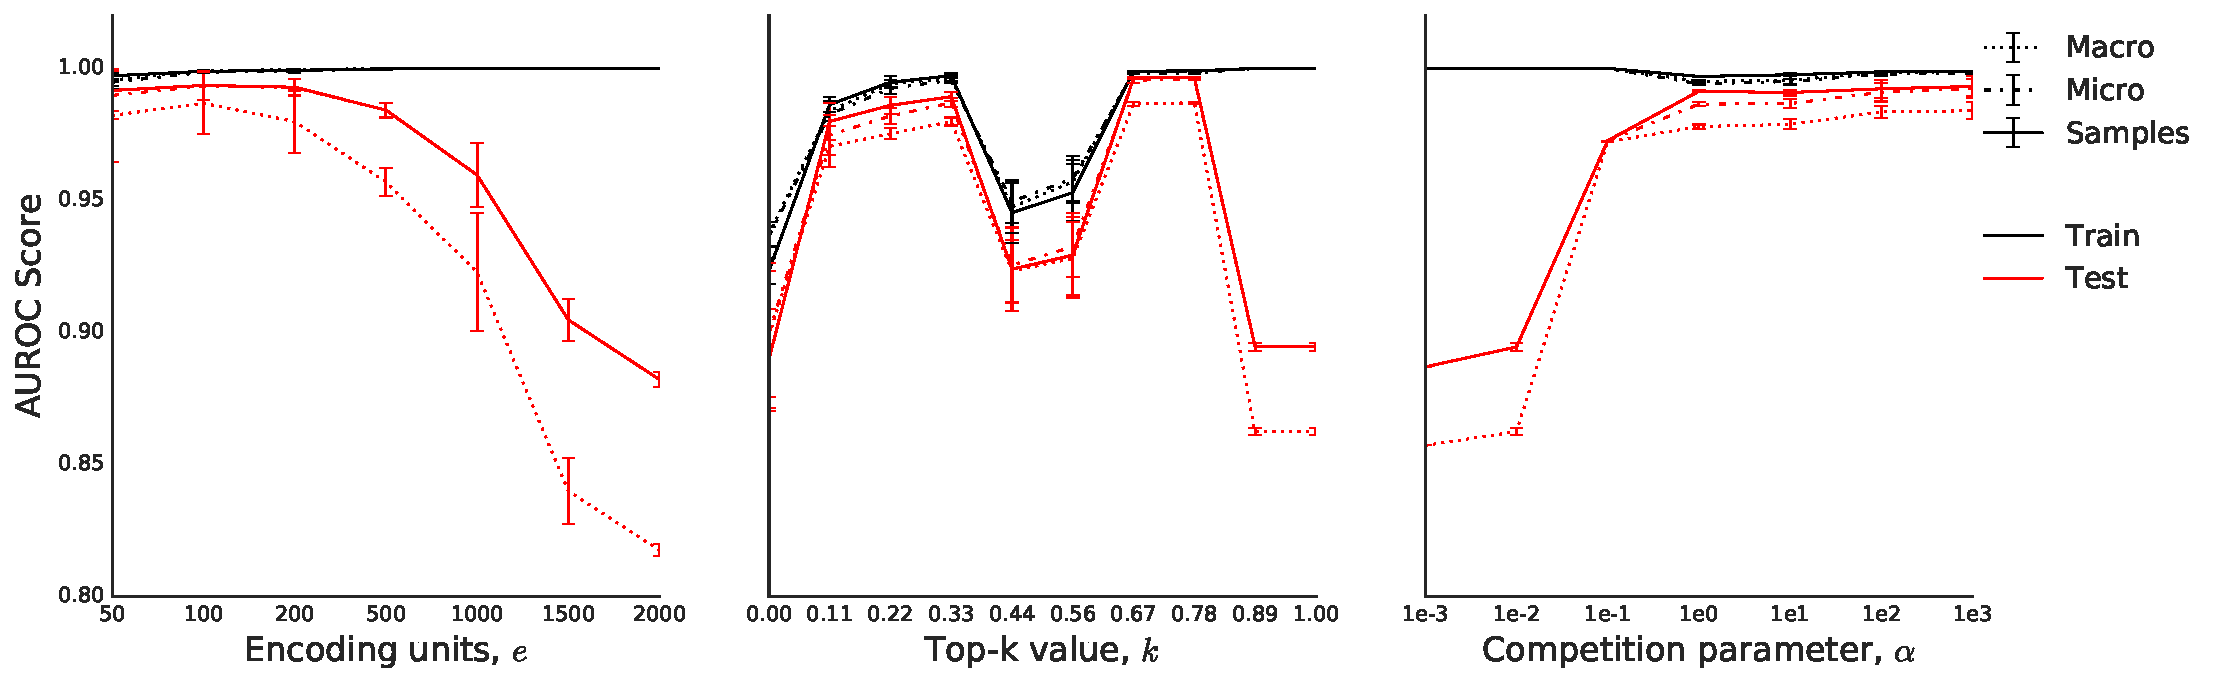
\includegraphics[width=0.95\textwidth]{ch04/hyperparams_genbase}
  \caption{Model behavior on the Genbase Dataset}
  \label{results:mc_char_genbase}
\end{figure}

\subsection{Key results for the mutually-competitive autoencoder}

Throughout this work, our main hypothesis states that the features extracted by
the proposed autoencoder are relevant, thus giving better predictions when
fed to a multilabel classifier. In this section, we will present key results
testing this claim.

\subsubsection{Examining feature relevance}

\par Decision trees were proven to provide reliable information regarding a
feature's importance during classification (\cite{kazemitbar2017variable}).
Thus, to quantify feature relevance, we trained a decision tree
$\mathcal{T}(\mathcal{X}, \mathcal{Y})$ to obtain a set of feature scores
$\mathcal{S} = \{s_{i}\}_{i=1}^{N}$ for each feature ${x}_{i}$. Then, we
normalized the scores between $0$ and $1$ and plotted their distribution on a
histogram. We performed this experiment for both raw attributes
$\mathcal{T}_{1}(\mathcal{X}=\mathbf{X}, \mathcal{Y}=\mathbf{Y})$ and
extracted features $\mathcal{T}_{2}(\mathcal{X}=\mathbf{X}^{\prime},
\mathcal{Y}=\mathbf{Y})$. Figure \ref{results:mc_score_distribution} shows
the feature score distribution for both datasets.

\begin{figure}[!h]
  \centering
  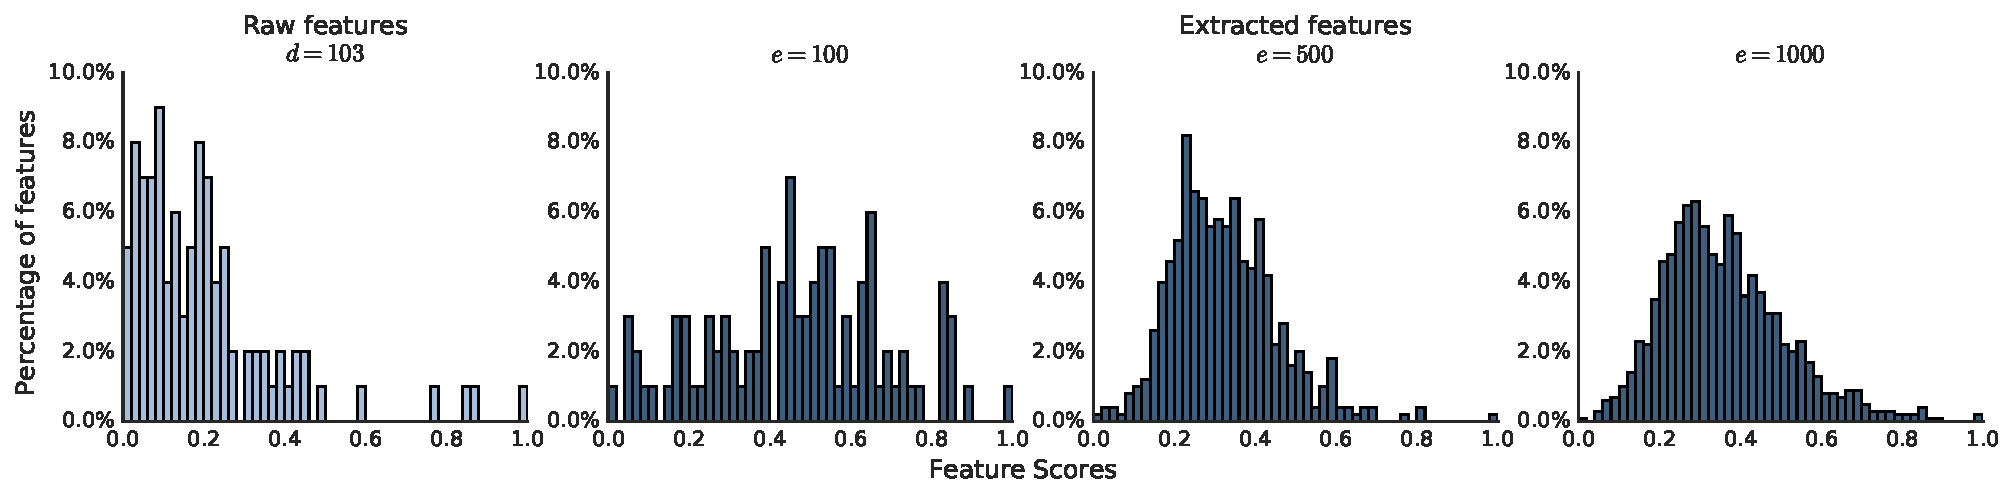
\includegraphics[width=0.95\textwidth]{ch04/fi_yeast}
  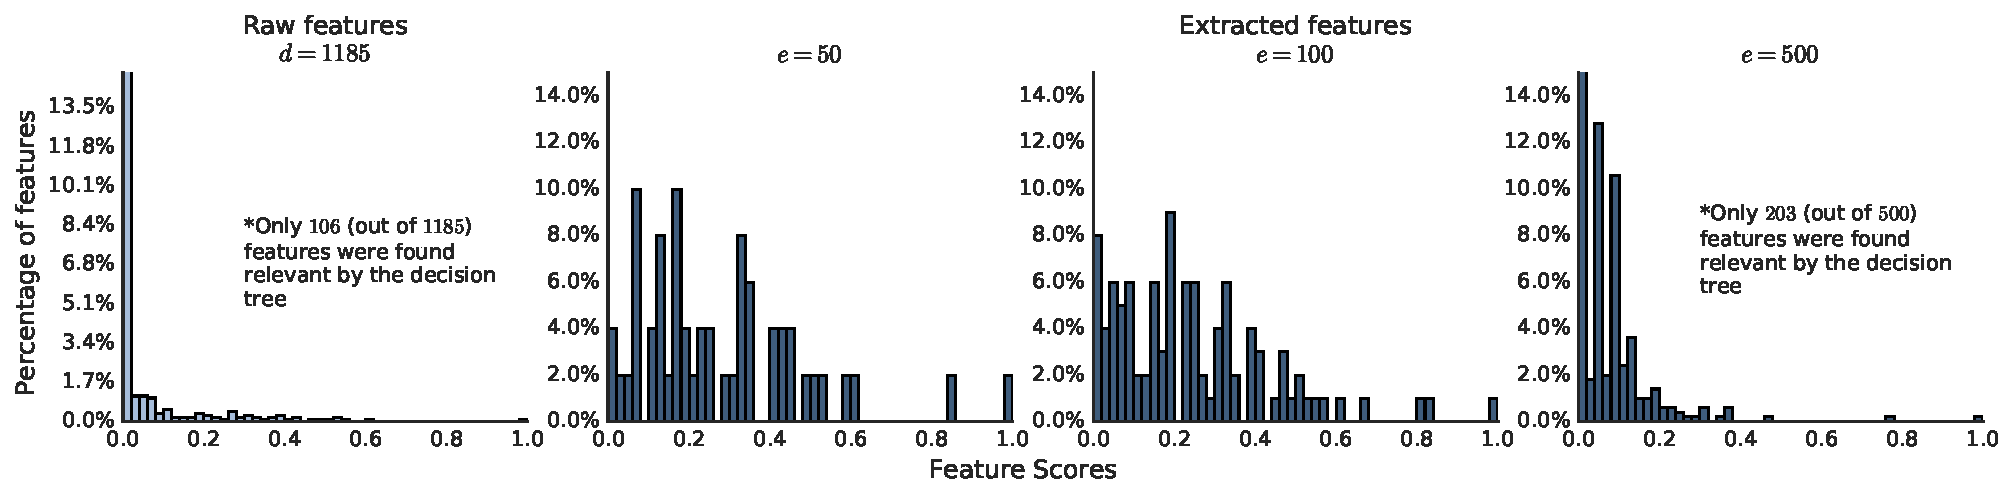
\includegraphics[width=0.95\textwidth]{ch04/fi_genbase}
  \caption[Feature score distribution for the two protein benchmarks]{
    Feature score distribution for both Yeast (\textit{top}) and Genbase
    (\textit{bottom}) datasets for different number of encoding units.
  }
  \label{results:mc_score_distribution}
\end{figure}

\par The feature score distribution for the raw attributes is colored
light-blue. It is evident that for both datasets, the distribution lies on
the lower value-range. This is especially true for Genbase, with only a small
fraction of features found relevant. This suggests that given a
classification task, the current feature space will not perform
well.\footnote{This is further validated by benchmark comparisons in later
experiments} However, the score distribution shifted to a higher-range upon
using the extracted features. This behavior is consistent for different
encoding units. This suggests that with respect to the classification task,
the extracted features are important and contributes well in achieving better
predictive performance.

\subsubsection{Assessing model quality}

This experiment serves as a ``sanity-check'' to test if the extracted
features are indeed suitable for classification. After obtaining new features
from the mutually-competitive autoencoder, they were used as input to a
BR-SVM classifier for prediction. Then, we drew Receiver Operating
Characteristic (ROC) and Precision-Recall (PR) curves as shown in Figure
\ref{results:mc_quality}. We plotted test set performance for the overall
model and for five (5) random labels for completeness.

\begin{figure}[!h]
  \centering
  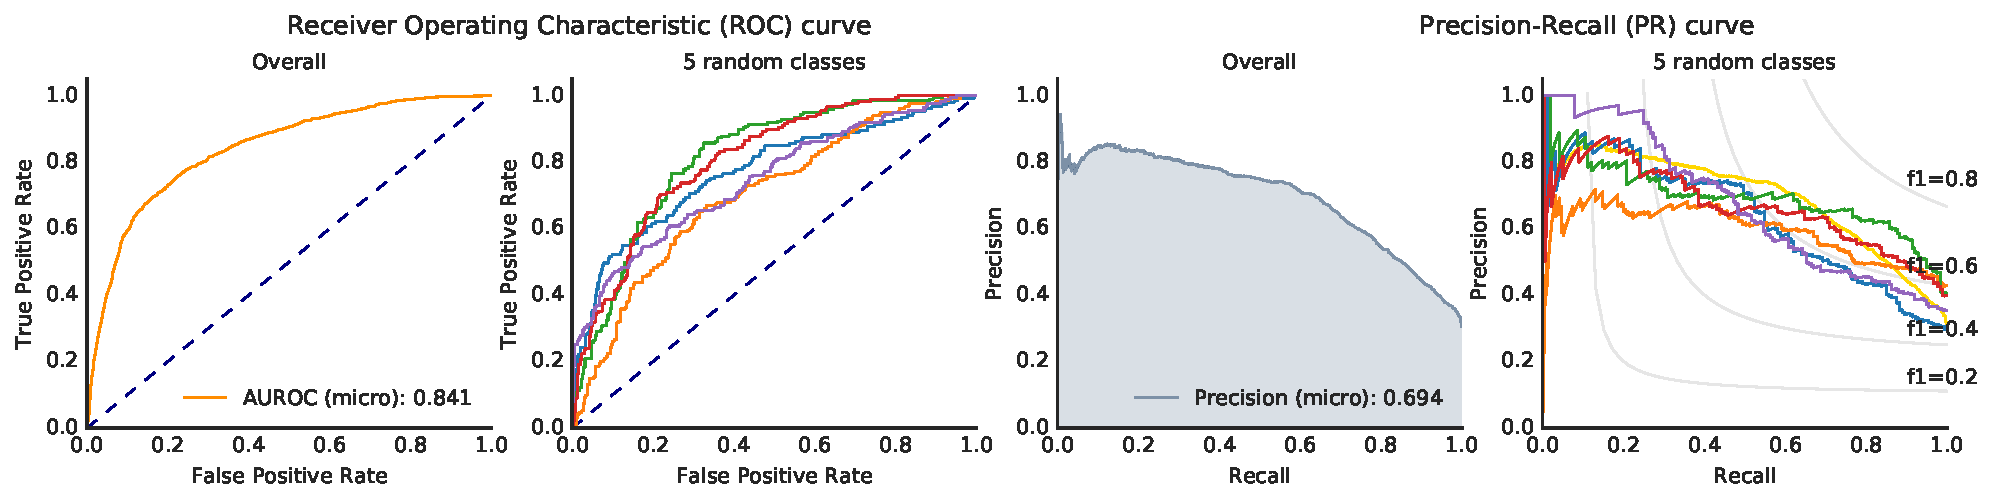
\includegraphics[width=0.95\textwidth]{ch04/ql_yeast}
  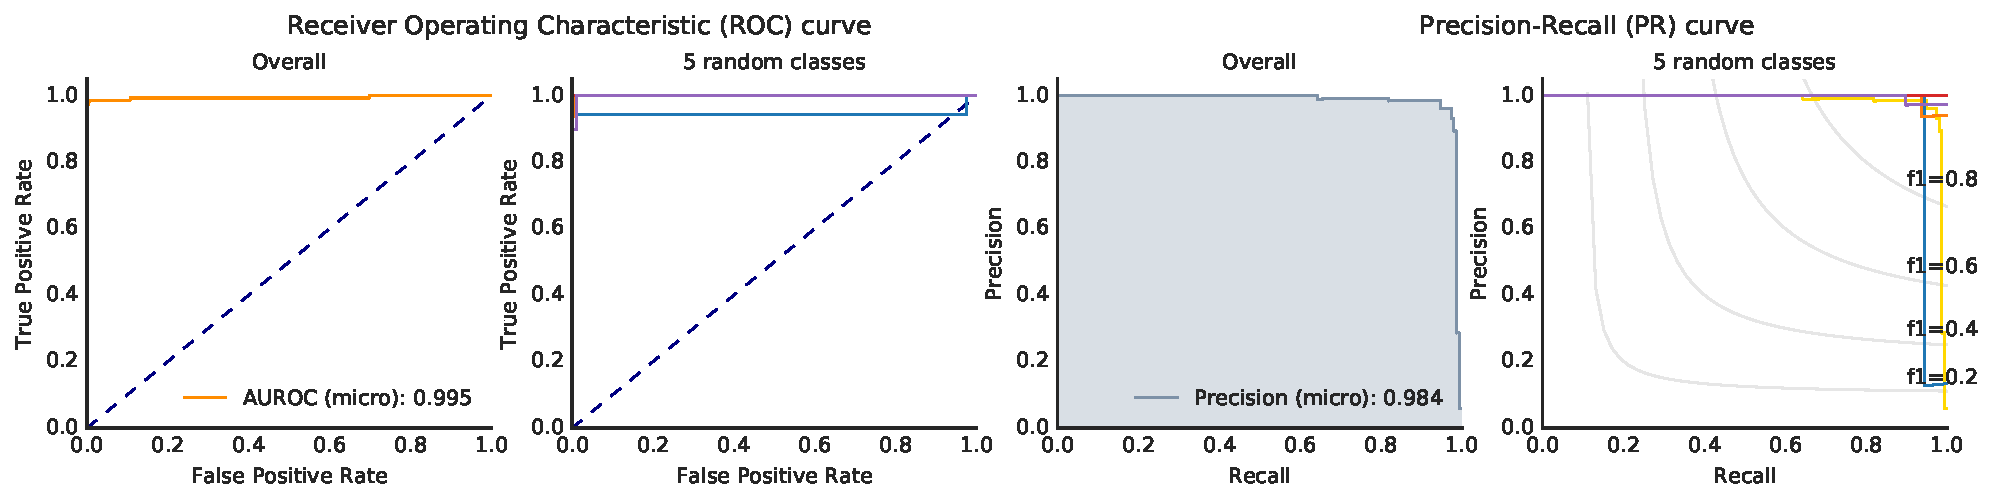
\includegraphics[width=0.95\textwidth]{ch04/ql_genbase}
  \caption[Receiver Operating Characteristic (ROC) and Precision-Recall (PR)
  curves for the two protein benchmarks]{
    Receiver Operating Characteristic (ROC) and Precision-Recall (PR) curves
    for both Yeast (\textit{top}) and Genbase (\textit{bottom}) datasets.
  }
  \label{results:mc_quality}
\end{figure}

\par The easiest way to interpret ROC curves is to check how far the curve is
from the dotted line.\footnote{This line represents the performance of a
random classifier. Only inside this scope, we will call this as the
baseline.} For both datasets, we can see that the orange curve is way above
the baseline, moreso with Genbase. This indicates that the classifier can
decently predict protein functions using the extracted features. On the other
hand, the PR curves reflect the precision-recall tradeoff for both datasets.
We can qualitatively gauge the optimal point where both precision and recall
are at their maximum by finding the vertex of the curve. For Yeast, this is
when Precision $P = 0.742$ and for Genbase, when $P=0.988$. In the next
section, we'll bring these results into context by comparing our model (i.e.,
feature extractor with the classifier) to other models in literature.

\subsubsection{Benchmark analysis}

\par In this experiment, we compared against similar techniques in literature.
We ran the models for ten (10) trials, and reported test set performance. In
addition, we performed post-hoc statistical tests to check if the differences
between groups are significant. Tables \ref{results:mc_benchmark_yeast} and
\ref{results:mc_benchmark_genbase} show the results.

\par Here, the baseline method corresponds to a model without feature
extraction. The raw attributes were directly fed to the BR-SVM classifier for
inference. This enables us to check if there is any performance difference
between the extracted features and the raw attributes. The ``Sig.'' column
indicates the extent in $\alpha$ in which the null hypothesis $H_{0}$ is
rejected. We implemented the Friedman's ranking test to compute for
$p$-values (\cite{friedman1937use, demsar2006statistical}). For Friedman's
test, $H_{0}$ states that there is no significant difference between groups.

\begin{table}[t]
%
\centering
\begin{threeparttable}
\caption{Benchmark analysis on Yeast dataset}
\label{results:mc_benchmark_yeast}
%
\begin{tabular}{@{}rr*{6}{l}@{}}
\toprule
        & & \multicolumn{5}{c}{Prediction Model\tnote{1}} \\ \cmidrule{3-7}
Metrics & Avg. & Baseline & M1 & M2 & M3 & Proposed\tnote{2} &
Sig.\tnote{3}\\
\midrule
AUROC & micro & \num{0.667(3)} & \num{0.666(2)} & \num{0.643(1)} &
\num{0.668(4)} & \hg \num{0.732(2)} & *** \\
        & macro & \num{0.655(3)} & \num{0.659(2)} & \hg \num{0.662(1)} &
        \num{0.648(2)} & \num{0.646(2)} & ** \\
        & sample & \num{0.670(3)} & \num{0.656(2)} & \num{0.643(1)} &
        \num{0.657(3)} & \hg \num{0.743(4)} & *** \\
F-score & micro & \num{0.548(4)} & \num{0.538(2)} & \num{0.530(1)} &
\num{0.579(3)} & \hg \num{0.629(3)} & *** \\
        & macro & \num{0.597(4)} & \num{0.603(2)} & \num{0.590(1)} &
        \num{0.613(2)} & \hg \num{0.630(2)} & *** \\
        & sample & \num{0.536(3)} & \num{0.524(2)} & \num{0.517(1)} &
        \num{0.572(3)} & \hg \num{0.609(4)} & *** \\
Hamming Loss & -- & \num{0.322(2)} & \num{0.343(2)} & \num{0.354(1)} &
\num{0.231(3)} & \hg \num{0.224(2)} & *** \\
\bottomrule
\end{tabular}
%
\begin{tablenotes}
        \footnotesize
    \item[1] M1: \cite{wang2013protein}, M2: \cite{chicco2014deep}, M3: \cite{miranda2017feature}
    \item[2] Feature ext.: $\{e=500,\alpha=10.0,k=0.6\}$, BR-SVM: $\{C=\num{1.00}, \gamma=\num{1.63e-3}\}$
    \item[3] Significance: *-$p\leq 0.1$, **-$p\leq 0.05$, ***-$p\leq 0.01$
\end{tablenotes}
%
\end{threeparttable}
%
\end{table}

\begin{table}[t]
%
\centering
\begin{threeparttable}
\caption{Benchmark analysis on Genbase dataset}
\label{results:mc_benchmark_genbase}
%
\begin{tabular}{@{}rrllllll@{}}
\toprule
        &       &  \multicolumn{5}{c}{Prediction Model\tnote{1}} \\ \cmidrule{3-7}
Metrics & Avg.  & Baseline       & M1             & M2             & M3               & Proposed\tnote{2}  & Sig.\tnote{3}\\
\midrule
AUROC     & micro    & \num{0.856(0)} & \num{0.987(0)} & \num{0.974(10)} & \num{0.987(1)}  & \hg \num{0.999(0)}  & ***  \\
        & macro    & \num{0.671(0)} & \num{0.992(0)} & \num{0.979(11)} & \num{0.983(1)}  & \hg \num{0.999(0)}  & ***  \\
        & sample    & \num{0.613(0)} & \num{0.950(0)} & \num{0.976(10)} & \num{0.988(1)}  & \hg \num{0.999(0)}  & ***  \\
F-score & micro    & \num{0.671(0)} & \num{0.887(1)} & \num{0.785(87)} & \num{0.962(11)} & \hg \num{0.986(7)}  & ***  \\
        & macro    & \num{0.716(0)} & \num{0.950(0)} & \num{0.892(40)} & \num{0.964(6)}  & \hg \num{0.992(2)}  & ***  \\
        & sample    & \num{0.760(0)} & \num{0.928(0)} & \num{0.810(95)} & \num{0.970(8)}  & \hg \num{0.989(6)}  & ***  \\
Hamming Loss   & --    & \num{0.041(0)} & \num{0.014(2)} & \num{0.035(17)} & \num{0.005(1)}  & \hg \num{0.002(0)}  & ***  \\
\bottomrule
\end{tabular}
%
\begin{tablenotes}
    \footnotesize
    \item[*] Values with $0.XXX(0)$ stdev. have deviations in the ten-thousandths place 
    \item[1] M1: \cite{wang2013protein}, M2: \cite{chicco2014deep}, M3: \cite{miranda2017feature}
    \item[2] Feature ext.: $\{e=30,\alpha=5.32,k=0.6\}$, BR-SVM: $\{C=\num{1.00}, \gamma=\num{1.24e-3}\}$
    \item[3] Significance: *-$p\leq 0.1$, **-$p\leq 0.05$, ***-$p\leq 0.01$
\end{tablenotes}
%
\end{threeparttable}
%
\end{table}


\par It is highly-evident that the mutually-competitive autoencoder performed
better in comparison to other models by a significant margin. It also
outperformed the Baseline across all metrics, validating our claim that using
extracted features\textemdash especially those from the proposed
autoencoder\textemdash can lead to better predictive performance. Lastly, we
conducted a post-hoc Bonferroni-Holm (\cite{holm1979simple}) test to compare
each model against each another using the results from both datasets. Table
\ref{results:mc_stats} shows this comparison. The $p$-values indicate that the
proposed model, when accounting for all metrics in both datasets, performs
significantly better than other techniques in literature.

\begin{table}[t]
%
\centering
\begin{threeparttable}
\caption{One-vs-All Overall Comparison\\using post-hoc Bonferroni-Holm Test\tnote{1}}
\label{results:mc_stats}
%
\begin{tabular}{@{}r*{3}{l}@{}}
\toprule
Proposed Model vs.                       & Z-statistic    & $p$-value         & Sig.\tnote{2} \\ \midrule
Baseline                                 & $4.54187$      & $0.00002$         & ***           \\
\cite{wang2013protein}                   & $3.28688$      & $0.00203$         & ***           \\
\cite{chicco2014deep}                    & $4.78091$      & $0.00001$         & ***           \\
\cite{miranda2017feature}                & $1.73308$      & $0.08308$         & *             \\ \bottomrule
\end{tabular}
\begin{tablenotes}
\footnotesize
\item[1] Friedman's test rejects $H_{0}$ with $\chi^{2}=\num{17.71730}$.
\item[2] Significance: *-$p\leq0.1$, **-$p\leq0.05$, ***-$p\leq0.01$
\end{tablenotes}
\end{threeparttable}
\end{table}


\subsubsection{Ablation tests}

\par In this experiment, we test if our modifications to the traditional
autoencoder are beneficial to the model's predictive performance.  We start
from a source configuration, then incrementally add components until we reach
the target configuration. We begin with a traditional autoencoder as our
source, then add the winner-take-all (WTA) and sparse (SL) operations until we
achieve the target architecture. For each step, we evaluate using the Area
under the ROC curve. Figure \ref{results:mc_ablation} shows the results.

\begin{figure}[t]
  \centering
  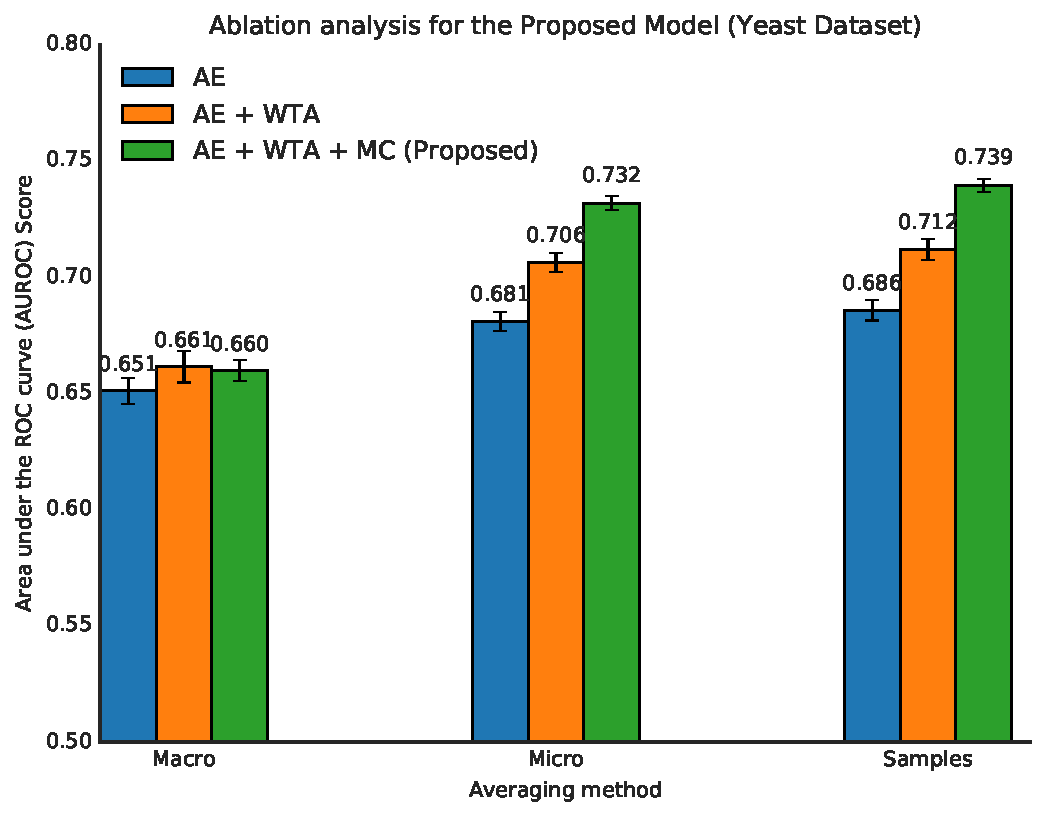
\includegraphics[width=0.38\textwidth]{ch04/ab_yeast}
  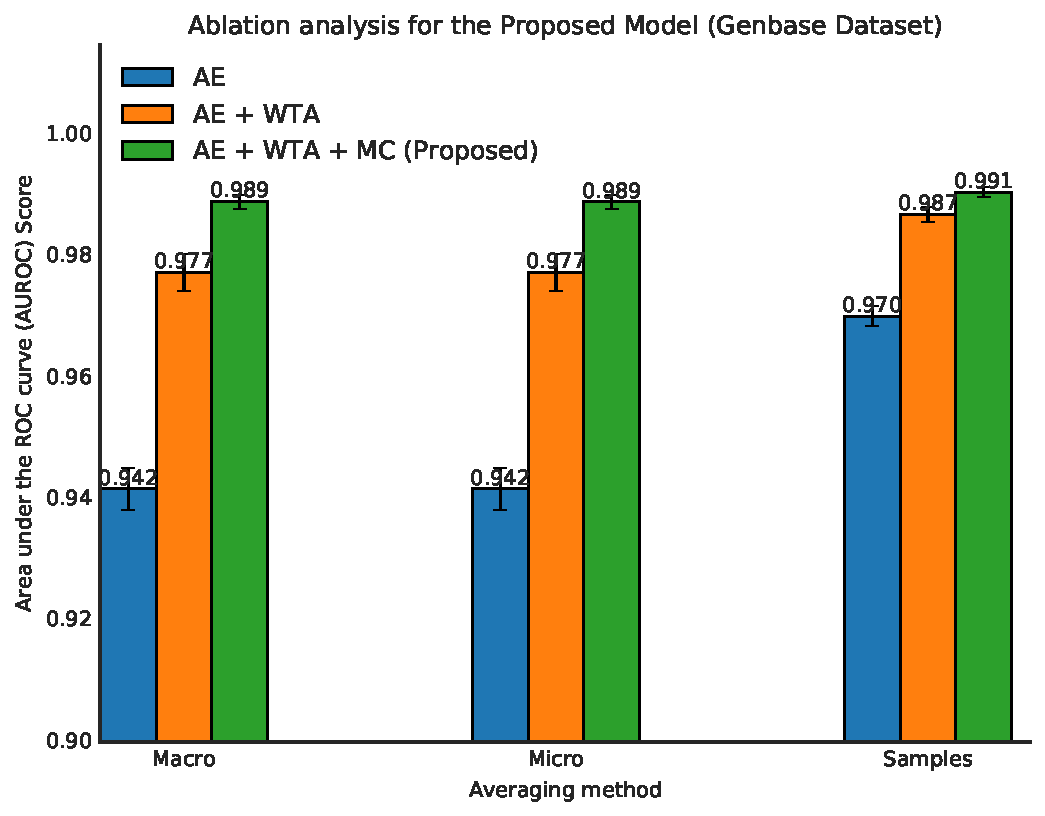
\includegraphics[width=0.38\textwidth]{ch04/ab_genbase}
  \caption[Ablation test results for the two protein benchmarks]{
    Ablation test results (Area under the ROC curve)
    for both Yeast (\textit{left}) and Genbase (\textit{right}) datasets.
  }
  \label{results:mc_ablation}
\end{figure}

\par It is evident that as we add components to the traditional autoencoder,
the performance of the predictor improves. There is a sharp increase from AE
upon addition of WTA, suggesting that the bottleneck improves model
performance. Winner-take-all keeps the highly-activated neurons, and using them
for feature extraction serves a beneficial purpose. More importantly, there is
also a performance increase when the sparse operation was added to the WTA
set-up. Manipulating the information flow has helped improve model accuracy,
and gave empirical weight to the efficacy of our method. Overall, the above
results prove that mutual competition is indeed essential to achieve high
predictive performance.

\section{Conclusion}
\label{MCConclusions}

\par To extract task-relevant and meaningful representations of data for
predicting protein functions, we designed a mutually-competitive autoencoder
architecture.  Our proposed method shares some similarities with the
traditional autoencoder, but has an additional layer consisting of
winner-take-all and sparse operations. Together, they encourage neurons that
best represent the input to be activated throughout training. We hypothesize
that the feature extractor should be able to derive task-relevant features, and
in consequence, boost a multilabel classifier's predictive performance.

\par The proposed autoencoder was tested on the Yeast and Genbase protein
benchmarks. First, we investigated how different hyperparameter settings
affect the model as a whole. The number of encoding units $e$ generally
depends on the dataset itself, with Yeast benefitting from overcomplete
configurations while Genbase for undercomplete architectures. However, the
top-$k\%$ neurons for the winner-take-all operation were seen to be optimal
at low values. This suggests that constraining the hidden layer helps
representation of data. Lastly, the intensity of competition, $\alpha$, is
helpful when set to a certain value. Very high values of $\alpha$ (in the
order of $10^{2}$ or $10^{3}$) only gives marginal returns. It is helpful to
note that finding values for $k$ and $\alpha$ is beneficial than setting
$k=1$ (keep all neurons) or $\alpha=0$ (no competition).

\par Next, we conducted experiments to test our claim. By training a decision
tree, the feature scores for the extracted features are much higher than
those of the raw attributes. Then, via a thorough comparison of the proposed
model with other techniques in literature, we saw that our model outperforms
most works by a significant margin. More importantly, the autoencoder has
greater performance than the baseline, further supporting our claim that
extracting features is more beneficial. Lastly, we performed ablation tests
to check if the modifications we've added to the traditional autoencoder
affects a model's predictive accuracy. The trendlines for both datasets show
that mutual competition in general benefits a classifier's performance.

\par This work validates the claim that extracting task-relevant features can
lead to better classification. In our case, we have demonstrated that the
mutually-competitive autoencoder performs task-relevant feature extraction.
The performance of the classifier when using the task-relevant features is
higher than just using raw attributes or extracted features from naive
methods.
